\documentclass{beamer}


\usepackage{amsmath,amsfonts,amssymb,amsthm, gensymb}
\DeclareMathAlphabet{\mathbbold}{U}{bbold}{m}{n}    

\usepackage[utf8]{inputenc}
 
 
%Information to be included in the title page:
\title{A Parallel in Time Method for Optimal Control}
\subtitle{Parareal-Based preconditioner for BFGS algorithm}
\author{Andreas Thune}
\date{2017}
 
\usetheme{Berlin}
 
\begin{document}
 
\frame{\titlepage}
\tableofcontents
\section{Problem}
\begin{frame}
\frametitle{Optimization with ODE constraints}

\begin{align*}
\min_{y,v} &J(y(t),v), \\
\textrm{subject to} \ &E(y(t),v)=0\quad t\in[0,T]
\end{align*}
\end{frame}
\begin{frame}
\frametitle{Adjoint approach to gradient evaluation}
\begin{align*}
\hat J'(v)=E_v^*p +J_v
\end{align*}
\begin{align*}
E_y^*p = J_y
\end{align*}
\end{frame}
\begin{frame}
\frametitle{Example problem}
\begin{align*}
J(y,v) = \frac{1}{2}\int_0^Tv(t)^2dt + \frac{\alpha}{2}(y(T)-y^T)^2 
\end{align*}
\begin{align*}
\left\{
     \begin{array}{lr}
       	y'(t)=ay(t) + v(t) \quad \textrm{for } \ t\in(0,T),\\
       	y(0)=y_0.
     \end{array}
   \right. 
\end{align*}
\end{frame}
%llllllllllllllllllllllllllllllllllllllllllllllll
\section{optimization}
\begin{frame}
\frametitle{Line search methods}
\begin{align*}
x^{k+1} = x^k -\gamma^k p^k
\end{align*}
\end{frame}
\begin{frame}
\frametitle{BFGS}
\begin{align*}
H^{k+1} = (\mathbbold{1}-\rho_kS_k\cdot Y_k)H^k(\mathbbold{1} -\rho_kY_k\cdot S_k) + S_k\cdot S_k
\end{align*}
\end{frame}
%llllllllllllllllllllllllllllllllllllllllllllllll
\section{PPC}
\begin{frame}
\frametitle{Quadratic penalty method}
\begin{align*}
\min_x f(x) \quad \textrm{subject to} \ c_i(x)=0 \quad i=1,...,N
\end{align*}
Transform constrained problem into unconstrained problem
\begin{align*}
f_{\mu}(x) = f(x) + \frac{\mu }{2}\sum_{i=1}^N c_i(x)^2 
\end{align*}
\end{frame}
\begin{frame}
\frametitle{Consistency}
\begin{align*}
\lim_{\mu\rightarrow\infty} v^{\mu}=v
\end{align*}
\end{frame}
\begin{frame}
\frametitle{Parareal-based preconditioner}
\begin{align*}
(v^{k+1},\Lambda^{k+1}) = (v^k,\Lambda^k) - \rho^kH^k \hat J'(v^k,\Lambda^k)
\end{align*}
\end{frame}
\begin{frame}
\frametitle{Virtual problem}

 \begin{align}
\bold J(y,\Lambda) = \frac{1}{2} x(\Lambda)^Tx(\Lambda), \label{non_lin_LS}
\end{align}
\begin{align}
x(\Lambda)=\left( \begin{array}{c}  
   \lambda_1 - \bold F_{\Delta T}(\lambda_0) \\ 
   \lambda_2 - \bold F_{\Delta T}(\lambda_1) \\
   \cdots  \\
   \lambda_{N-1} -\bold F_{\Delta T}(\lambda_{N-1}) \\
   \end{array}  \right).
\end{align}

\end{frame}
%llllllllllllllllllllllllllllllllllllllllllllllllll
\section{consistency}
\begin{frame}
\frametitle{Consistency}
\begin{figure}[!h]
\centering
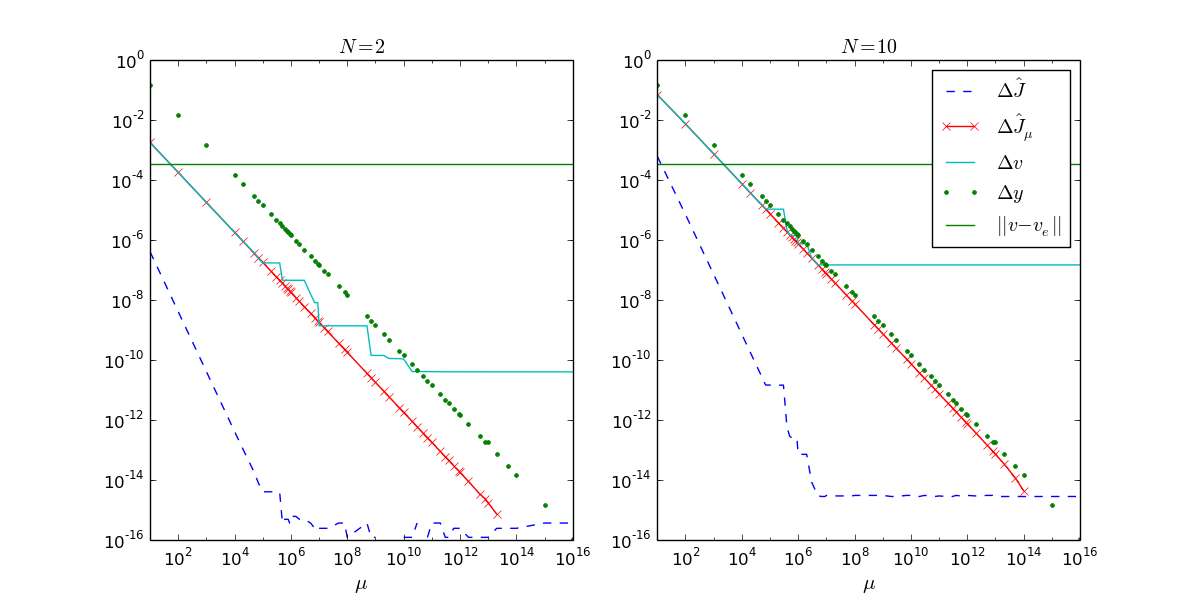
\includegraphics[scale=0.4]{consistency1.png}

\end{figure}
\end{frame}
%llllllllllllllllllllllllllllllllllllllllllllllllll
\section{Experiments}
\begin{frame}
hei hallo
\end{frame}
\end{document}

